\documentclass[16pt]{article}
\usepackage{graphicx}
\font\myfont=cmr12 at 40pt

\title{EX01}

\date{}

\author{        Daronhil Mauricette \\
                Student ID: z20375dm \\
		COMP23111 \\
		2017 - 2018 }
\begin{document}
\maketitle
\newpage

\begin{figure}
  \centering
  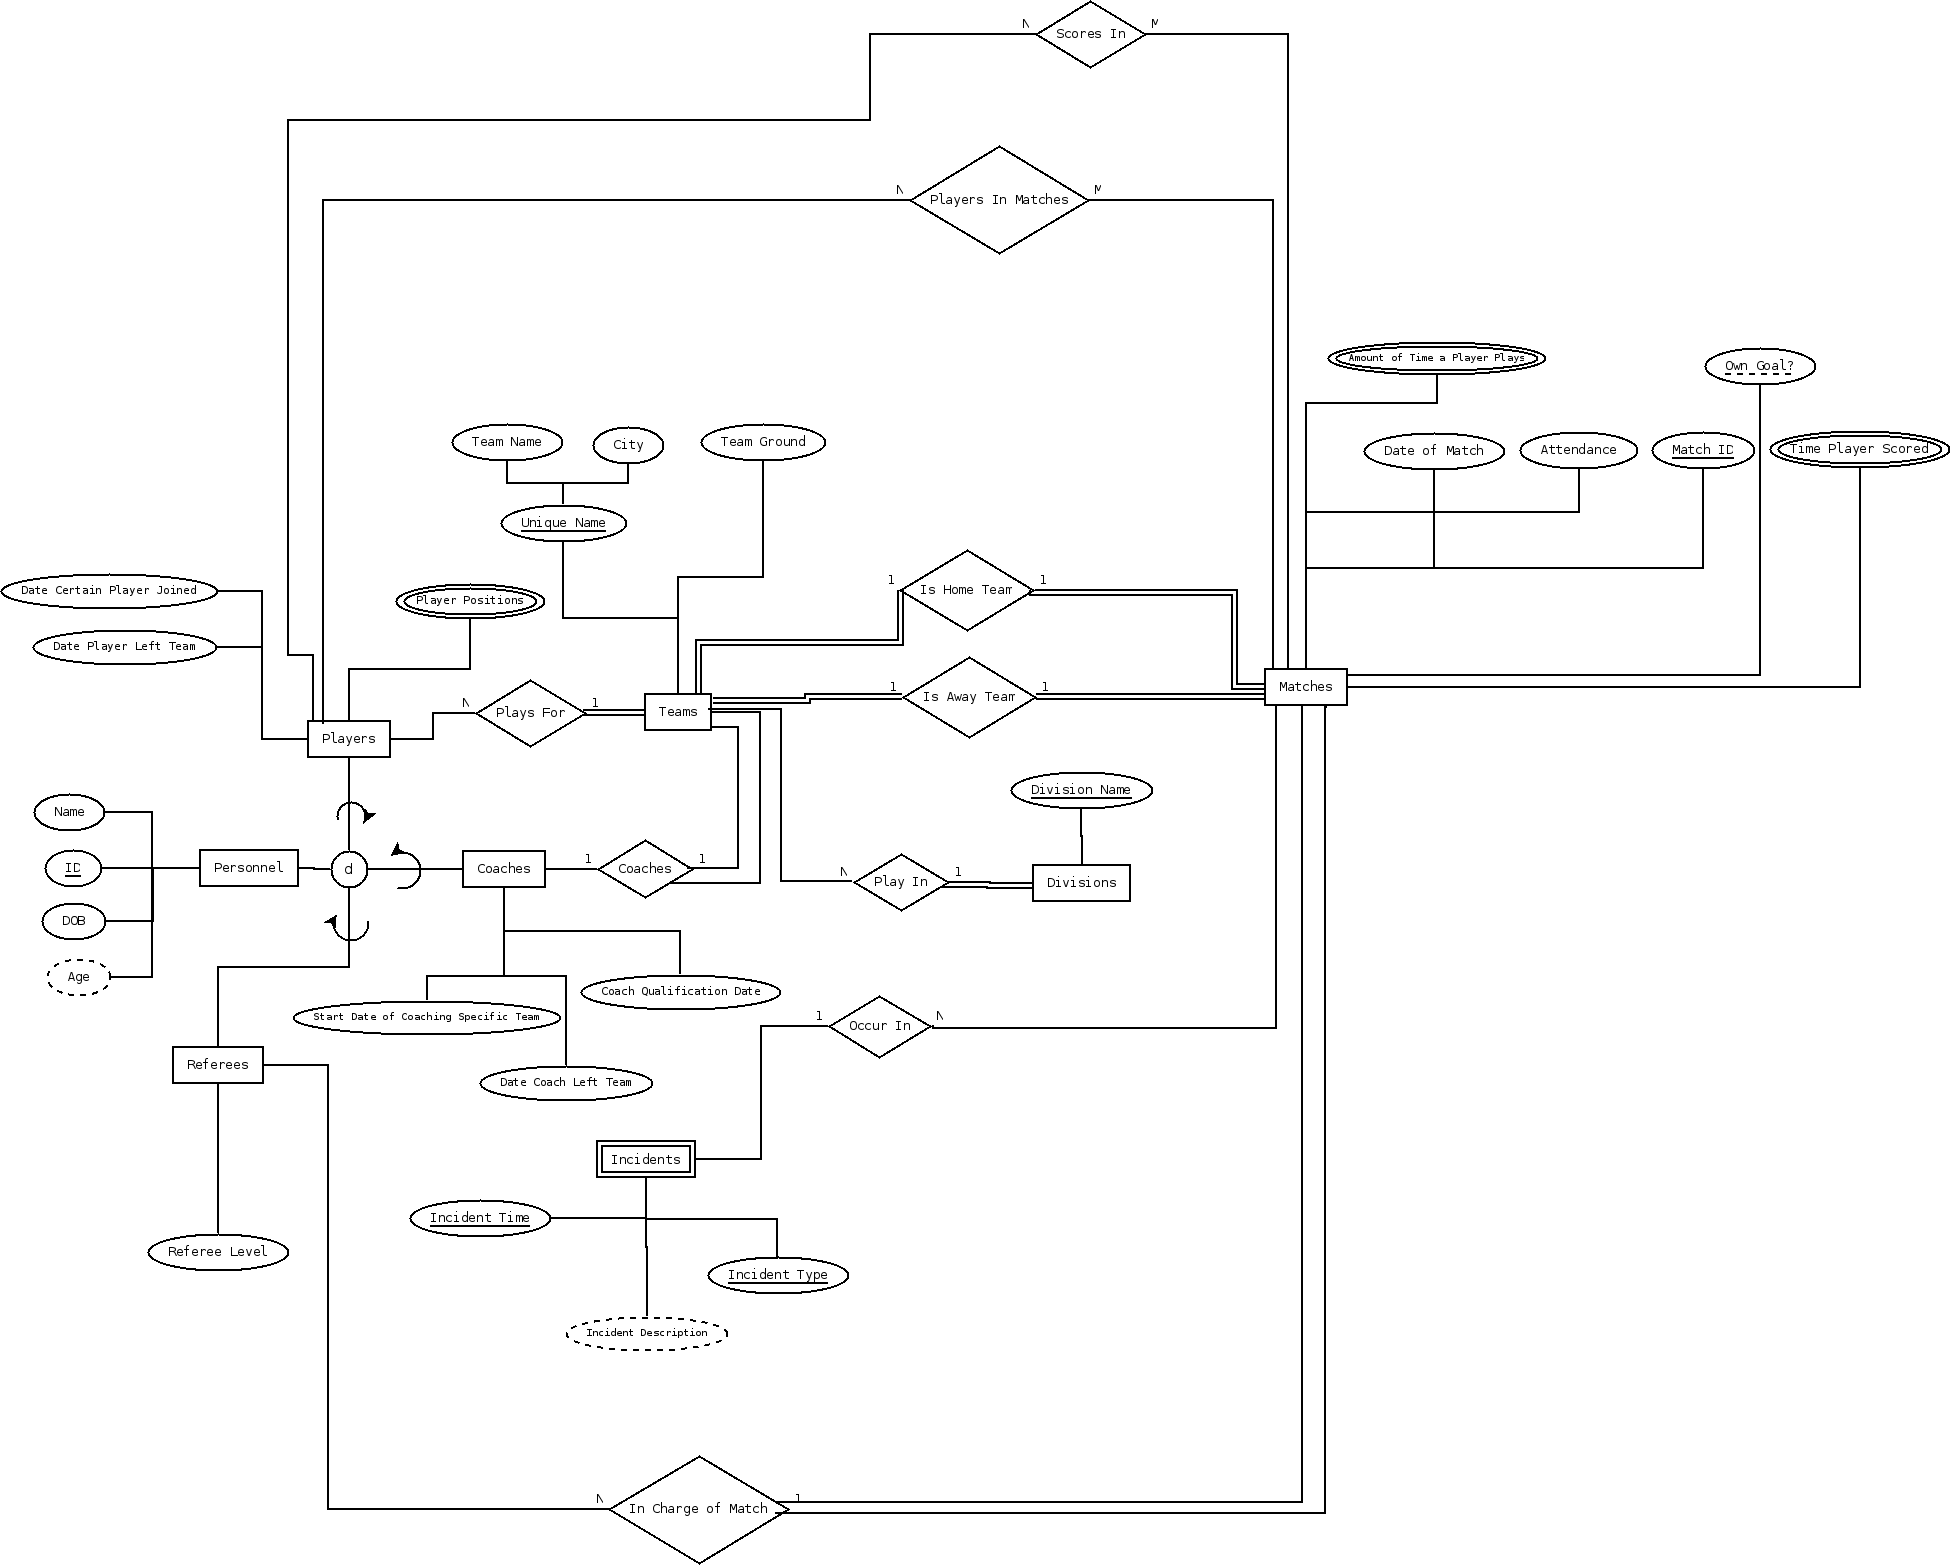
\includegraphics[scale=1,bb=0 0 30 30]{EX01-z20375dm.png}
  \centerline{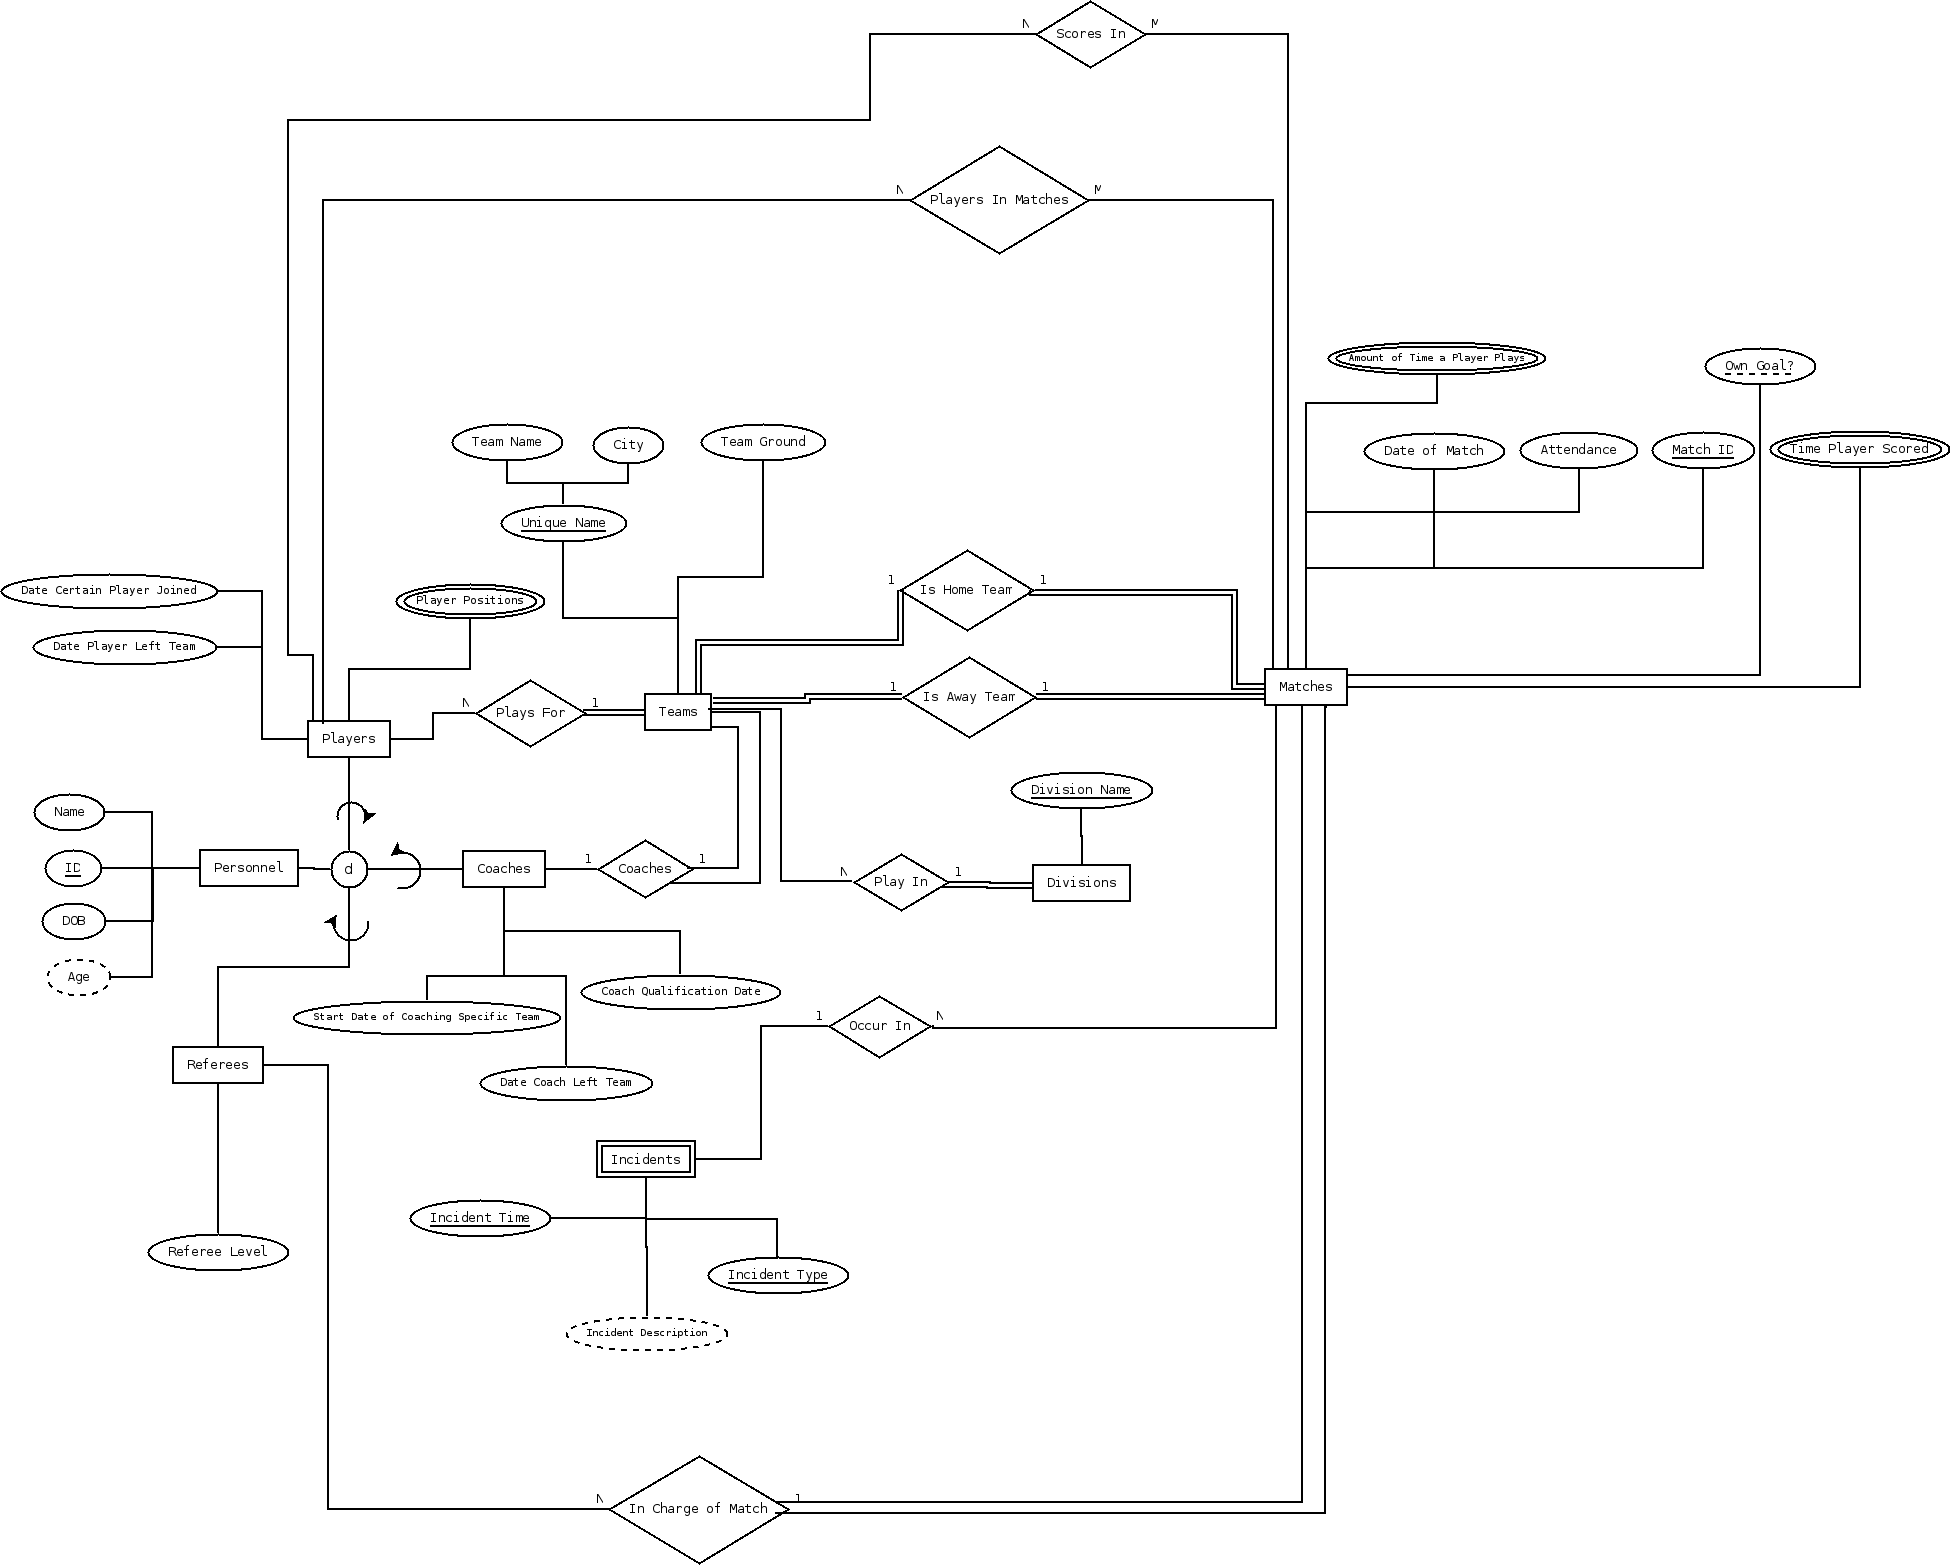
\includegraphics[width=17cm]{EX01-z20375dm.png}}
  \caption{The DRS of a database of a sports league}
  \label{fig:DRS1}
\end{figure}

\newpage
\section{Comments/Assumptions}
My first assumption is that I assume the DRS is done correctly, but regardless
of that fact I thought this was a very straight forward task to complete. It
may have taken some time but I understand what I have created. The only part I 
may have some issues with is the division of entities. Other than that I feel 
sure of my work.

\end{document}
